\documentclass{../TexTemplate/myslide}
\usepackage[slide,table,python]{../TexTemplate/mypackage}
\hypersetup{colorlinks=true,linkcolor=black,urlcolor=blue}
\usepackage{xcolor}

\renewcommand{\thefootnote}{\fnsymbol{footnote}}

\title[ToolsSeminar]{Tools Seminar}
\subtitle{Week 8 - Deep Learning}
\author[chhzh123]{Hongzheng~Chen}
\date[Mar 16, 2020]{Mar 16, 2020}

\begin{document}

\begin{frame}
\titlepage
\end{frame}

\begin{frame}
\tableofcontents
\end{frame}

\section{Introduction}
\begin{frame}
\sectionpage
\end{frame}

\begin{frame}{AI Milestones}
% Major Milestones of Artificial Intelligence from 1949 to 2018
% https://medium.com/@angelapowell/major-milestones-of-artificial-intelligence-97d42bb5714c
\begin{itemize}[<+->]
\item 1950, Alan Turing proposed the famous Turing test
\item 1955, John McCarthy created the term ``artificial intelligence'' (1971 Turing award)
\item 1997, IBM's Deep Blue beat world chess champion Garry Kasparov
\item 2011, IBM Watson defeated two champions at quiz show Jeopardy
\item 2012, Jeff Dean and Andrew Ng used unsupervised learning to train neural network which learned to recognize cats
\end{itemize}
\end{frame}

\begin{frame}{AI Milestones (Cont.)}
\begin{itemize}[<+->]
\item 2012, AlexNet achieved an error rate of only 16\% in \href{http://image-net.org/challenges/LSVRC/2012/results.html}{ImageNet Large Scale Visual Recognition Challenge}
\begin{itemize}
	\item Alex Krizhevsky, Ilya Sutskever, Geoffrey Hinton (University of Toronto)
	\item 2 GPU, a week, halved the error rate
	\item \textbf{Open the era of deep learning}
\end{itemize}
\item 2015, Kaiming He (MSRA) proposed ResNet which made machine see better than human (3.6\% error rate in ImageNet)
\item 2016, Google DeepMind's AlphaGo defeated 9-dan Go master Lee sedol by 4:1
\begin{itemize}
	\item Firstly proposed deep reinforcement learning
\end{itemize}
\item 2018, Google \href{https://www.blog.google/products/search/search-language-understanding-bert/}{BERT} model achieved the state-of-the-art performance in 11 NLP tasks
\end{itemize}
\end{frame}

\begin{frame}{ImageNet \& Deep Neural Network}
ImageNet [Feifei Li, Stanford] Large Scale Visual Recognition Challenge
\begin{center}
\begin{tabular}{cccccc}\hline\hline
 & LeNet & AlexNet & VGG & GoogleLeNet & ResNet\\\hline
\# of Layers & 5 & 8 & 19 & 22 & \textbf{152}\\\hline
Top 5 Error & N/A & 16.4\% & 7.3\% & 6.7\% & 3.57\%\\\hline
Year & 1994 & 2012 & 2014 & 2014 & 2015\\\hline
\end{tabular}
\end{center}
This is why it's called ``\textbf{deep}'' learning\\
\end{frame}

\begin{frame}{2018 Turing Award}
\href{https://awards.acm.org/about/2018-turing}{2018 Turing Award}: Geoffrey Hinton, Yoshua Bengio, Yann LeCun
\\\bigskip
\begin{quote}
``for conceptual and engineering breakthroughs that have made deep neural networks a critical component of computing''
\end{quote}
\begin{itemize}
	\item Geoffrey Hinton: Backpropagation, Boltzmann Machines, Improvements to Convolutional Neural Network (CNN)
	\item Yoshua Bengio: Probabilistic models of sequences, High-dimensional word embeddings and attention, Generative adversarial networks (GAN)
	\item Yann LeCun: CNN, backprop, Broadening the vision of neural networks
\end{itemize}
\end{frame}

\begin{frame}{Impetus of Deep Learning}
Looking back, we may know what leads to the boom of DL in 2010s
\begin{itemize}
	\item Large amount of labeled \textbf{data}: ImageNet
	\item Improvement of \textbf{hardware}: GPU $\to$ GPGPU (general-purpose GPU)
	\item Improvement of \textbf{algorithms}: deep networks, dropout
\end{itemize}
\end{frame}

\begin{frame}{Introductory Books and Courses}
\begin{columns}
\begin{column}{0.5\linewidth}
\begin{itemize}
\item Feifei Li, \href{http://cs231n.github.io/}{Stanford cs231n}: Convolutional Neural Networks for Visual Recognition (highly recommended!)
\item Chris Manning, \href{https://web.stanford.edu/class/archive/cs/cs224n/cs224n.1194/}{Stanford cs224n}: Natural Language Processing with Deep Learning
\item Ian Goodfellow, \href{https://www.deeplearningbook.org/}{Deep Learning}\\
\href{https://github.com/exacity/deeplearningbook-chinese}{Chinese version}
\end{itemize}
\end{column}
\begin{column}{0.5\linewidth}
\begin{figure}
\centering
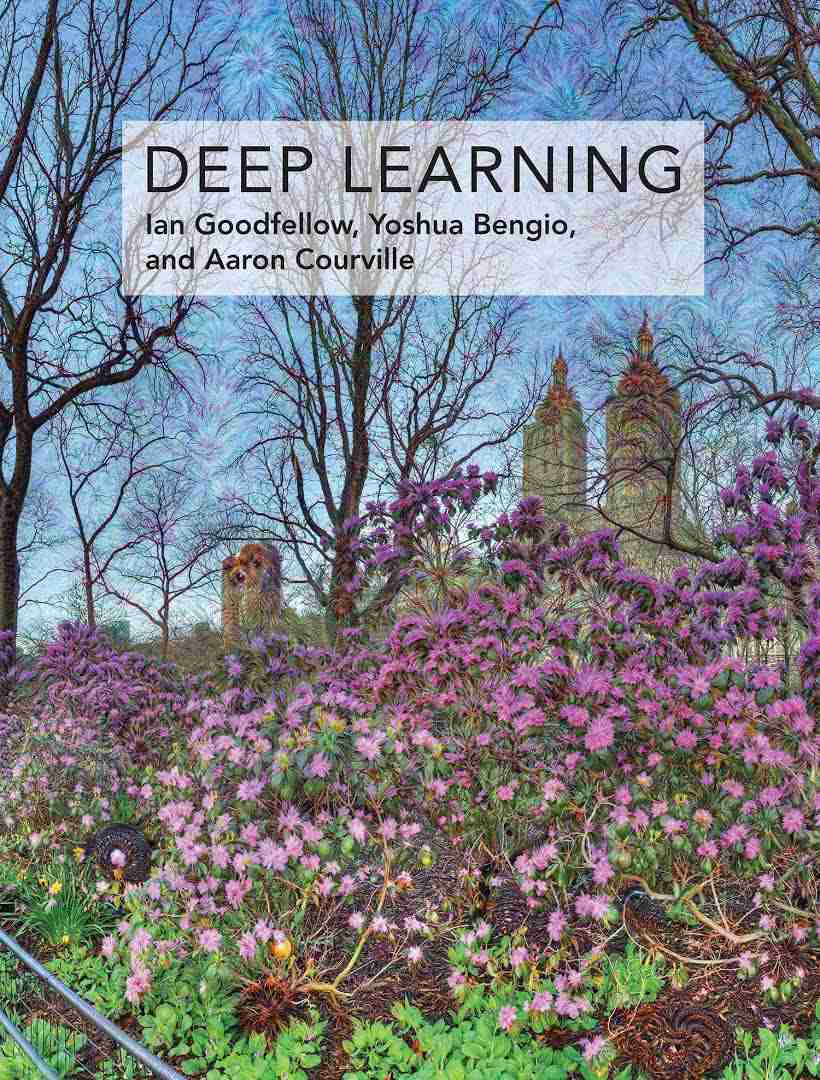
\includegraphics[width=0.8\linewidth]{fig/dl_book.jpeg}
\end{figure}
\end{column}
\end{columns}
\end{frame}

\section{Deep Learning}
\begin{frame}
\sectionpage
\end{frame}

\begin{frame}{Linear Regression}
Recall the linear regression problem
\[y=\vw^\T\vx+b=\bmat{\vx^\T & b}\bmat{\vx\\1}=\vtheta^\T\vx\]
To minimize loss function (MSE)
\[\min_{\vtheta} L(\vtheta)=\frac{1}{m}\sum_{i=1}^m(y_i-\vw^\T\vx_i-b)^2\]
But linear function can only deal with linearly separable problems
\begin{figure}
\centering
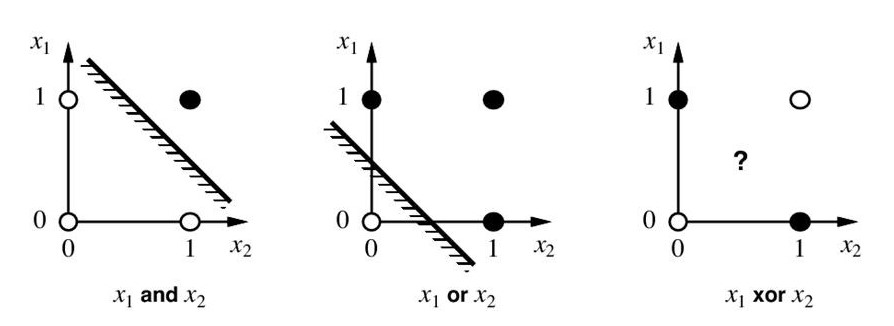
\includegraphics[width=0.8\linewidth]{fig/linearly-separable.jpeg}
\end{figure}
\end{frame}

\begin{frame}{Powerful Models}
Can we build a model that is powerful enough to represent all the functions?
\begin{itemize}
	\item $f(\text{image})=\text{location}$
	\item $f(\text{question})=\text{answer}$
	\item $f(\text{speech})=\text{text}$
	\item $\cdots$
\end{itemize}
\pause
Actually, in ML area, we have built decision tree, SVM, etc., but they usually need feature engineering and are not flexible
\end{frame}

\begin{frame}{Neuron Model}
We can refer to our brain and see how we learn
\begin{figure}[H]
\centering
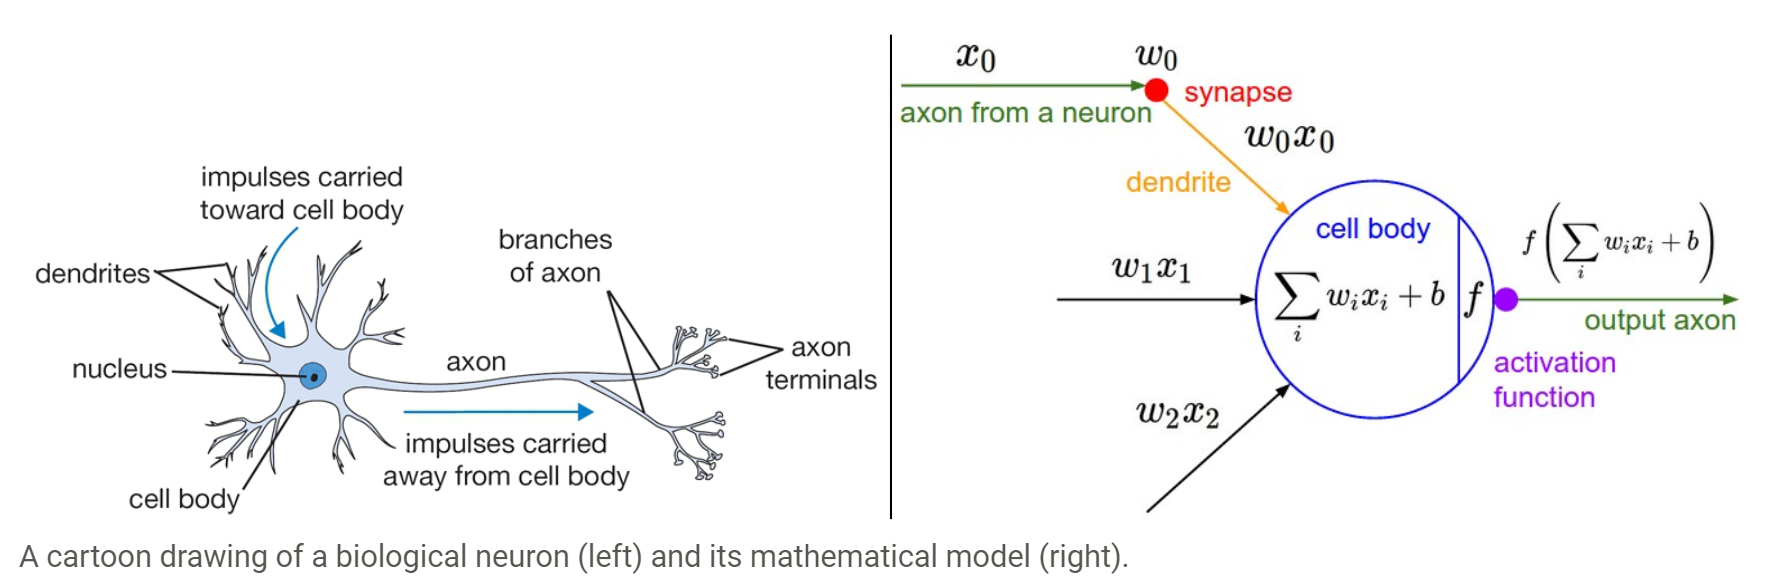
\includegraphics[width=\linewidth]{fig/neuron_model.png}
\caption*{\small Fig source: \url{http://cs231n.github.io/neural-networks-1/}}
\end{figure}
\pause
A neuron is just a linear model with activation function!
\end{frame}

\begin{frame}{Activation Function}
Used to add non-linear part to the model, enabling it to approximate much more complex functions
\begin{figure}
\centering
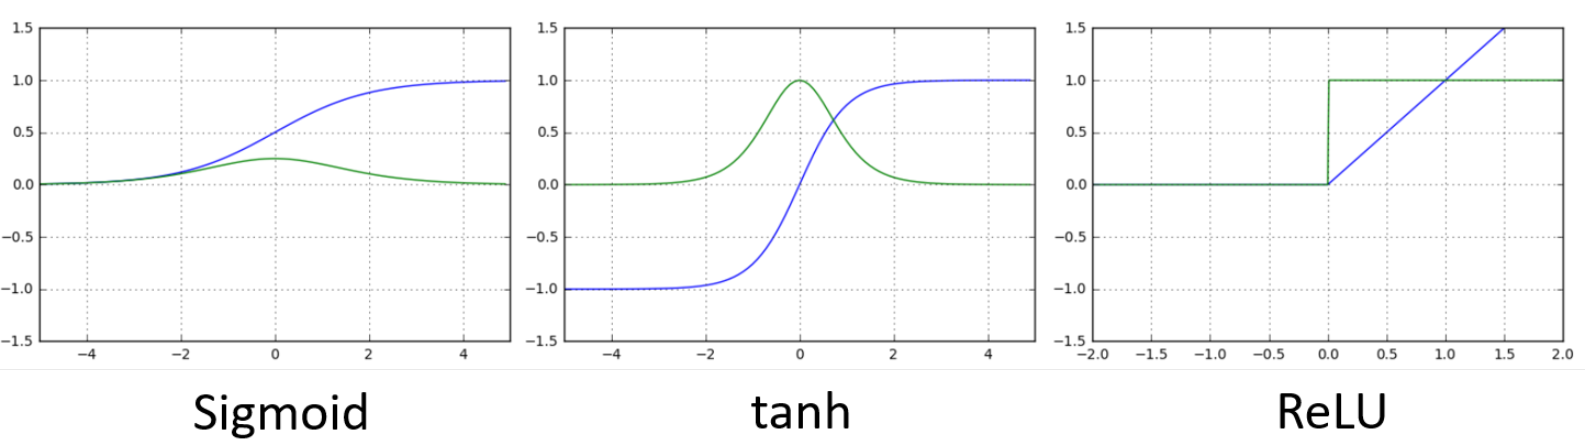
\includegraphics[width=0.8\linewidth]{fig/activation_function.png}
\end{figure}
\begin{itemize}
	\item Sigmoid: $g(z)=1/(1+\ee^{-z})$ (S curve)
	\item Tanh: $g(z)=\tanh(z)$
	\item ReLU (Rectified Linear Unit): $g(z)=\max(0,z)$, can avoid gradient vanishing
\end{itemize}
\end{frame}

\begin{frame}{From one to more}
Only one neuron can do limited things, what about more?
\begin{itemize}
	\item More neurons in width:
	\begin{quote}
	A feed-forward network with a single hidden layer containing a finite number of neurons can approximate continuous functions on compact subsets of $\rn$.\\
	\hfill --- \href{https://en.wikipedia.org/wiki/Universal_approximation_theorem}{The Universal Approximation Theorem}
	\end{quote}
	The question is that the theorem does not tell us how many neurons we need
	\pause
	\item More neurons in depth: We have multi-layer perceptron (MLP) --- the basic model of nowadays deep learning!
\end{itemize}
\end{frame}

\begin{frame}{Multi-Layer Perceptron (MLP) / Fully-connected NN}
\begin{figure}
\centering
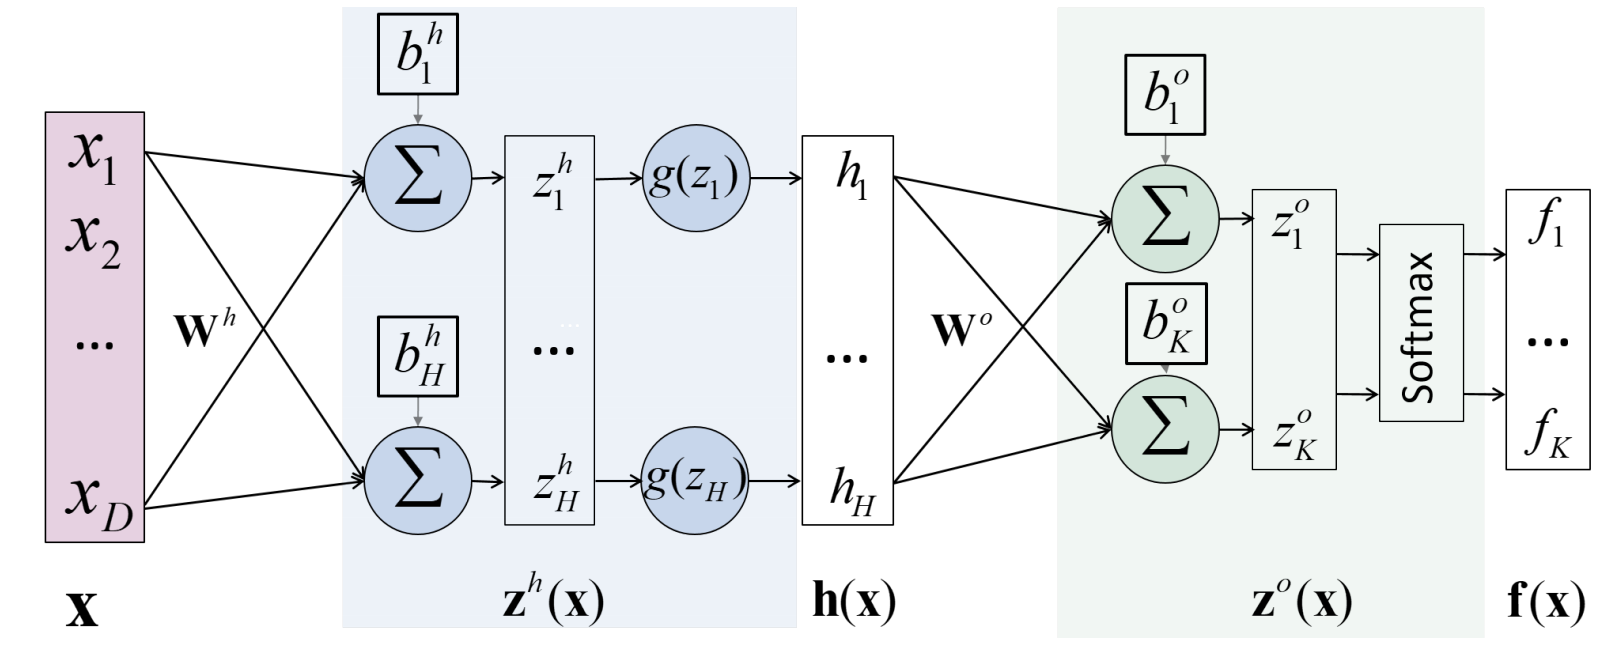
\includegraphics[width=0.8\linewidth]{fig/mlp.png}
\end{figure}
\begin{itemize}
	\item Input layer: $\vx$
	\item Hidden layer: $h(\vx)=g(\vz^h(\vx))=g(W^h\vx+\vb^h)$
	\item Output layer: $f(\vx)=\sigma(\vz^o(\vx))=\sigma(W^o h(\vx)+b^o)$
\end{itemize}
* Softmax function: change output to probability ($K$-dimensional)
\[\sigma(\vz)_j=\frac{\ee^{z_j}}{\sum_{k=1}^K\ee^{z_k}}\]
\end{frame}

\begin{frame}{Classifier Training}
\begin{itemize}
	\item Find optimal parameters $\vtheta^*$ of a classifier $\vy=f(\vx;\vtheta)$
	\item Rule: given input $\vx$, classifier output $f(\vx;\vtheta)$ should be as close to the ideal output as possible
\end{itemize}
\begin{figure}
\centering
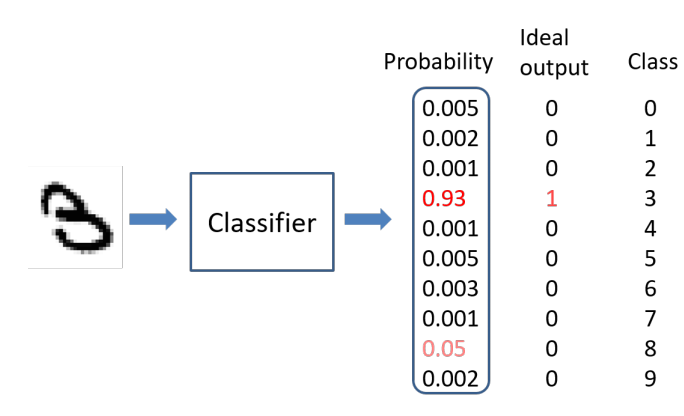
\includegraphics[width=0.8\linewidth]{fig/classifier.png}
\end{figure}
\end{frame}

\begin{frame}{Classifier Training}
Use MSE or other loss function
\[\min_{\vtheta} \frac{1}{N}\sum_{i=1}^N\norm{f(\vx_i;\vtheta)-y_i}_2^2\]
Use gradient descent to optimize parameters
\[\vtheta^{(k+1)}=\vtheta^{(k)}-\alpha\nabla_{\vtheta} L(\vtheta)\]
About how to optimize the above function on NN (backpropagation), please read \url{http://cs231n.github.io/optimization-1/}
\end{frame}

\begin{frame}{Different Kinds of NN}
\begin{itemize}
	\item \href{https://ujjwalkarn.me/2016/08/11/intuitive-explanation-convnets/}{CNN} (convolutional NN): CV
	\begin{itemize}
		\item Pooling / subsampling
		\item Dropout
		\item Residual block
	\end{itemize}
	\item RNN (recurrent NN): NLP
	\begin{itemize}
		\item LSTM
		\item GRU
	\end{itemize}
	\item GAN (generative adversarial network): Image generation
\end{itemize}
\end{frame}

\section{Frameworks}
\begin{frame}
\sectionpage
\end{frame}

\begin{frame}{Deep Learning Frameworks}
Framework: A large package consisting of lots of deep learning primatives/operators, and users can easily call them by API
\begin{itemize}
	\item Google: \href{https://www.tensorflow.org/}{Tensorflow} (commonly used in industry)
	\begin{itemize}
		\item Static computation graph
		\item Jeff Dean
	\end{itemize}
	\item Facebook: \href{https://pytorch.org/}{PyTorch} (commonly used in academics)
	\begin{itemize}
		\item Dynamic computation graph
		\item Yangqing Jia, Caffe
	\end{itemize}
	\item Amazon: MXNet
	\begin{itemize}
		\item Tianqi Chen (UW $\to$ CMU)
	\end{itemize}
\end{itemize}
* We focus on \textbf{PyTorch} in this seminar
\end{frame}

\begin{frame}{PyTorch}
PyTorch: A Python-based scientific computing package
\begin{itemize}
	\item A replacement for NumPy to use the power of GPUs
	\item A deep learning research platform that provides maximum flexibility and speed
\end{itemize}
Since it is highly embedded in Python, PyTorch is very Pythonic and easy-to-use
\end{frame}

\subsection{Installation}
\begin{frame}{Pytorch Installation}
Firstly check if your computer has discrete graphics card (GPU)
\begin{figure}
\centering
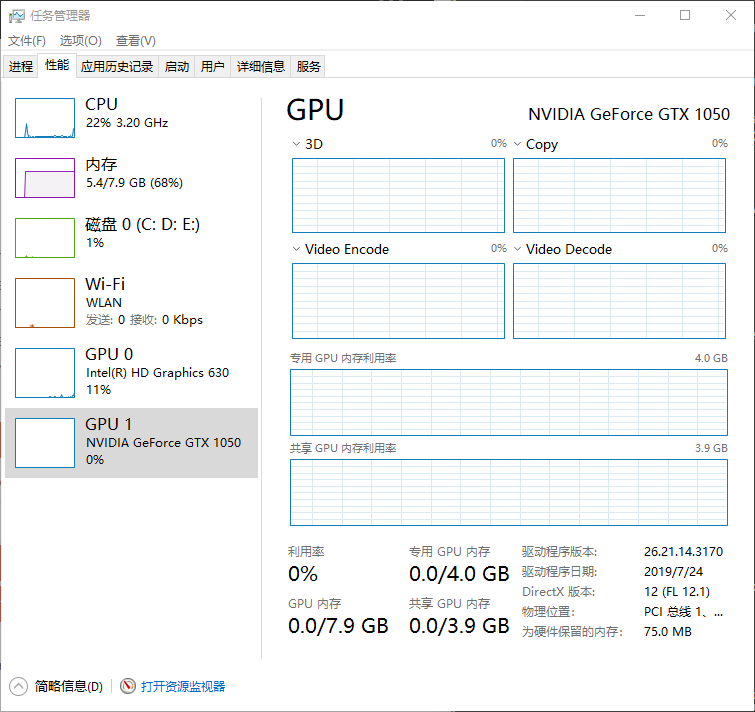
\includegraphics[width=0.45\linewidth]{fig/gpu-monitor.png}
\end{figure}
Install Nvidia driver: \url{https://zhuanlan.zhihu.com/p/54350088}
\begin{itemize}
	\item \href{https://developer.nvidia.com/cuda-10.1-download-archive-base}{CUDA 10.1}
	\item \href{https://developer.nvidia.com/cudnn}{cuDNN 7}: \href{https://docs.nvidia.com/deeplearning/sdk/cudnn-install/index.html}{Installation guide}
\end{itemize}
\end{frame}

\begin{frame}[fragile]{Pytorch Installation}
Select your configuration on this \href{https://pytorch.org/}{website} and run the installation command
\begin{itemize}
	\item Windows: Need to install Anaconda first
	\item WSL does not support GPU! Do NOT install Pytorch on WSL!
	\item Mac does not support GPU too (if you do not have external interface)!
\end{itemize}
e.g. For Windows with no GPUs
\begin{lstlisting}
pip install torch==1.4.0+cpu torchvision==0.5.0+cpu -f https://download.pytorch.org/whl/torch_stable.html
\end{lstlisting}
Check if GPU works correctly by
\begin{lstlisting}[language=python]
import torch
print(torch.cuda.is_available())
\end{lstlisting}
\end{frame}

\subsection{Tutorials}
\begin{frame}[fragile]{Tutorials}
PyTorch has very detailed documentations, make the best of them!
\begin{itemize}
	\item Tutorials: \url{https://pytorch.org/tutorials/}
	\item Chinese tutorials: \url{https://pytorch.apachecn.org/}
	\item Documentation / API: \url{https://pytorch.org/docs/stable/index.html}
	\item \href{https://pytorch.org/tutorials/beginner/deep_learning_60min_blitz.html}{Deep Learning with PyTorch: A 60 Minute Blitz}
	\begin{itemize}
		\item \href{https://pytorch.apachecn.org/docs/1.0/deep_learning_60min_blitz.html}{Chinese version}
		\item You can download the \verb'.ipynb' file or directly run on \href{https://colab.research.google.com/}{Colab}
	\end{itemize}
\end{itemize}
\end{frame}

\section{Summary}
\begin{frame}
\sectionpage
\end{frame}

\begin{frame}{Summary}
\begin{itemize}
	\item Introduction
	\item Deep Learning Framework: PyTorch
	\begin{itemize}
		\item Once you get in some trouble concerning PyTorch, you can search \href{http://pytorch.org/docs/master/index.html}{the Docs of PyTorch} for details. Alternatively you can try to find if there are similar problems on \href{https://discuss.pytorch.org/}{\emph{PyTorch Discuss}}.
	\end{itemize}
	\item Get through cs231n!
\end{itemize}
\end{frame}

\end{document}